\documentclass[conference]{IEEEtran}
\IEEEoverridecommandlockouts

\usepackage{color} %red, green, blue, yellow, cyan, magenta, black, white
\definecolor{mygreen}{RGB}{28,172,0} % color values Red, Green, Blue
\definecolor{mylilas}{RGB}{170,55,241}

% The preceding line is only needed to identify funding in the first footnote. If that is unneeded, please comment it out.
\usepackage{cite}
\usepackage{amsmath,amssymb,amsfonts}
\usepackage{algorithmic}
\usepackage{graphicx}
\usepackage{textcomp}
\usepackage{appendix}
\usepackage{xcolor}
\usepackage{listings}
\usepackage{fancyhdr}
\usepackage{float}
\usepackage{mathtools}
\DeclarePairedDelimiter{\ceil}{\lceil}{\rceil}
\def\BibTeX{{\rm B\kern-.05em{\sc i\kern-.025em b}\kern-.08em
    T\kern-.1667em\lower.7ex\hbox{E}\kern-.125emX}}
\begin{document}

\thispagestyle{fancy}
\cfoot{}
\renewcommand{\headrulewidth}{0pt}
\renewcommand{\footrulewidth}{0pt}
\pagestyle{fancy}
\rfoot{\thepage}
\title{SSY-135 Project part 2}


\author{\IEEEauthorblockN{Group E:}
\and
\IEEEauthorblockN{Oskar Claeson}
\and
\IEEEauthorblockN{Erik Tilly}
\and
\IEEEauthorblockN{Yuling Zhang}
\and
\IEEEauthorblockN{Haitham Babbili}
}

\maketitle

\section{Introduction}

The objective of this report is to increase the understanding of wireless transmission systems and in particular orthogonal frequency division multiplexing (OFDM) systems. This is done through designing and simulating an OFDM communication system in Matlab. A study of how the system behaves over two different channels is made. The two channels that were simulated are an additive white Gaussian noise (AWGN) channel and a time-varying frequency selective channel known as Rayleigh fading. This paper illustrates the method of designing such an OFDM system and evaluates the performance of said system. The evaluation of the system includes different plots and scatter-plots to provide a ground to discuss topics such as Symbol Error Rate (SER), Signal to Noise Ratio (SNR), the effects of cyclic prefix and more.




\section{Ofdm communication design and evaluation}
%OFDM technology has been introduced in most of the wireless network systems due to efficiency in the frequency spectrum. The technology is based on dividing the mainstream transmitted signals into many sub-stream signals carried over multi-subchannels. This achieves a higher data rate and eliminates the inter symbol interference(ISI), that if symbol time has chosen more than delay spread and coherent bandwidth for each subchannel much less than coherent bandwidth of the channel. Since OFDM uses modulation and multiplexing, QPSK modulation was implemented in this project. For multiplexing, this modulated signal goes throw buffer then separated to columns due to number of subcarriers. That means serial to parallel independent signal. Then transfer this signal into time domain by using Inverse fast Fourier transform (IFFT). 


 OFDM technology has been introduced in most of the wireless network systems due to efficiency in the frequency spectrum. The technology is based on dividing the mainstream transmitted signals into many sub-stream signals carried over multi-subchannels. This achieves a higher data rate and introduces higher importance in eliminating the inter symbol interference(ISI), which is why cyclic prefix is needed in the system. As modulation QPSK modulation was implemented before creating OFDM symbols. Which is done by Creating vectors of length N containing QPSK symbols and the implement cyclic prefix to them and after that convert it to the time domain by using Inverse fast Fourier transform (IFFT) which is the computational version of inverse discrete Fourier transform (IDFT) that you can see in equation \ref{IDFT}.


\begin{equation}
x(n)= \frac{1}{\sqrt{N}}\sum_{n=0}^{N-1} X(k) \exp{\frac{j2\pi kn}{N}}  \label{IDFT}
\end{equation}
where x(n) is the n-time signal value, X(k) is the spectral value, n is the time index, k is frequencies index and N length of the sequence.
The value of $N= 2^p$ where $p = \log_{2}(N)$ and N is even number.



\subsection{Determining the parameters}

The amount of taps the channel used is set such that it covers all paths. In this project, the delay spread is $5.4 \mu s$ and sample time $T_s = \frac{1}{bandwidth} = 1 \mu s$. Therefore the amount of channel taps $L$ is calculated according to equation \ref{tap} to be 6: 

\begin{equation}
    L \geq \frac{\tau_{DS}}{T_s}
    \label{tap}
\end{equation}

In order to trick the receiver, the data is periodic a set of the last symbols which are added to the start of the data sequence. This set of symbols are called cyclic prefix. To avoid Inter-Symbol Interference (ISI), the length of the cyclic prefix, denoted $N_{cp}$, need to be long enough to cover the total delay spread of the channel. If it is too short, then samples from a previous OFDM symbol may interfere with the newly transmitted samples. The relation between the number of channel taps and cyclic prefix length is shown below in equation \ref{NcpL}.

\begin{equation}
    N_{cp} \geq L-1
    \label{NcpL}
\end{equation}

For a lower complexity of the DFT, N should be power of two. During an OFDM symbol transmission over the channel, which should be close to constant to make the equalization at the receiver more accurate. Therefore, this sets a constraint on the sample length N. Theoretically, the constraints are set according to equation \ref{N}, which means that the total length of the OFDM symbol is much shorter than the coherence time of the channel. If assuming that a factor of $10$ corresponds to much smaller, then the limiting value of $N+N_{cp}$ can be calculated according to equation \ref{Nlim} which in this case equals to approximately 1000. This means that the theoretical maximum N as a power of 2 is $N = 512$. However, in the simulations, we noticed that the system could handle larger N without error occurring but to avoid long simulation times and not underestimated the channel, the length $N$ was set to 128.

\begin{equation}
   (N + Ncp)f_DT_s \ll 1 
   \label{N}
\end{equation}

\begin{equation}
    N+Ncp=\frac{0.1}{f_DT_s}
    \label{Nlim}
\end{equation}

The noise power spectrum density $N_0$ given for the project had the unit $[W/Hz]$. To make sure it has the correct unit for power, W, it is calculated according equation \ref{N0}. Where the bandwidth is given as two-sided.

\begin{equation}
    N_0 = 2 \times 2.07\times10^{-20}\times \frac{bandwidth}{2} \quad [W]
    \label{N0}
\end{equation}

In the transmitter part of the simulation, the symbol modulation was chosen to be a QPSK modulation as mentioned before. These symbols have an energy constraint $\mathbf{E}\{|s_k^m|^2\} = E$. Where the value of E can be related to the average transmit power times the symbol time according to equation \ref{E}. As an example: if $P=0.1 W$ and $T_s= 10^-6 s$, then $E$ is calculated as $E=10^{-7} J$
 
\begin{equation}
    E = P \cdot T_s
    \label{E}
\end{equation} 


\subsection{OFDM system design}

In the transmitter a OFDM symbol are created by building a vector with QPSK symbols with the length N and apply the IFFT operation to the vector to get it in the time domain. Then they are multiplied with $\sqrt{N}$ to normalize it according to equation \ref{design:transmitter}.  
\begin{equation}
     x[i] = \sqrt{N} \cdot \mathrm{IFFT(s)}
     \label{design:transmitter}
\end{equation}

After that, the cyclic prefix is implemented by copying the $N_{cp}$ first QPSK symbols and place a copy of them at the end of the vector. This makes it possible to manage it as a periodic signal, however this also increases the length of the vector to $N+N_{cp}$. Then this vector is sent through the channel and this process is repeated M times. 

When the signal arrives at the receiver, the first step is to remove the cyclic prefix. This is achieved by removing the $N_{cp}$ last QPSK symbols that has been received. The channel affects the signal both with rotation and amplitude. This is taken into consideration by taking an estimation of the channel and then remove it in the frequency domain. After that the signal is mapped with maximum likelihood. Since the QPSK symbols are random generated, they are equiprobable, hence, they are mapped to the symbol with the minimum distance.   



\section{Simulation over different channels}

\subsection{AWGN channel}
Firstly, the transmitter is created as a simple QPSK modulated sample sequence of N samples. These are then inversely discrete Fourier transformed to time domain and the cyclic prefix is added. The OFDM symbol is then put through the channel.
The AWGN channel is described as $\mathit{c_0(nT_s) = 1}$ and $\mathit{c_{l \neq 0}(nT_s) = 0 }$, $\forall{n}$. To simulate this in Matlab, the received signal is not equalized as this channel, c, does not introduce rotation nor scaling. However, the effects of the path loss is multiplied and random samples from a complex Gaussian distribution is added to the transmitted signal. This do introduce some scaling and can be seen in the scatter plots corresponding to the AWGN channel simulation shown in Appendix \ref{SCA_AWGN}. The receiver then simply checks which quadrant the received symbols are placed in the IQ-plane and chooses the QPSK symbol corresponding to that quadrant.


\subsection{Time-varying frequency selective channel}

The transmitter works the same way as for the AWGN channel simulation.
In this project, the provided function Fading\_channel.p is used to generate the time-varying frequency selective channel $\mathit{c_l(nT_s)}$. This channel distorts the amplitude and phase of the signal. When running the signal through the channel function, an estimation of the channel is also provided. When the OFDM symbol time is much shorter than the coherence time of the channel, then the first row of this channel estimation can be seen as the time domain response of the fading channel. After the signal has gone through the channel, in the same way as for AWGN channel simulation, the path loss effect and noise is added. The received signal is discrete Fourier transformed back to frequency domain to obtain the samples of the form $y_n = C_n\cdot s_n + w_n$, where C is related to the FFT of the time domain response of the channel. In order to remove the effects of the channel, the received samples are equalized, which is done by dividing y with C. These equalized samples are shown in scatter plots located in Appendix \ref{SCA_fading}. To recover the symbols correctly, the ML estimate boils down to minimizing the distance between the received symbols and the QPSK constellation points. The effective data rate of the system over the OFDM system is calculated to be approximately 3.85 Gbit/s according to following equation, where $bits\_per\_symbol=2$ for QPSK:
\begin{equation}
    r = (N/(N + N_{cp}))\cdot f_c\cdot bits\_per\_symbol
\end{equation}

\subsection{Energy vs SER}
To demonstrate the relation between the SNR and SER of the system, a SER vs SNR plot for the two channels were created. These are shown in figures \ref{SERfading} and \ref{SERawgn}. The simulation is a verification of how the SER corresponds to specific SNRs when using the Fading channel and AWGN channel. The simulated values are also compared to theoretical values of AWGN SER, which is created according to equation \ref{theo}.

\begin{equation}
    SER = 2\cdot \big Q \Bigg(\sqrt{\frac{E(i)\cdot pathloss}{N_0}}\Bigg) \label{theo}
\end{equation}

\begin{figure}[H]
    \centering
    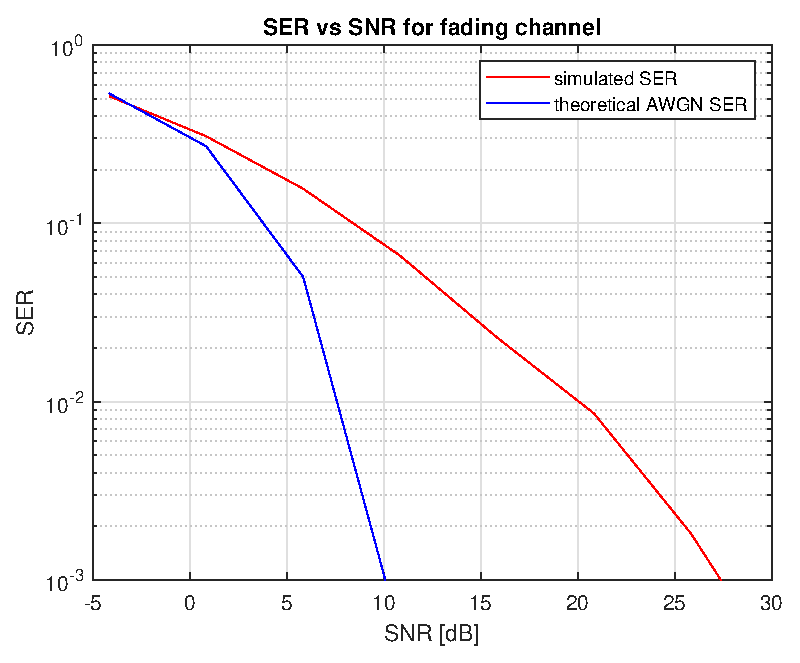
\includegraphics[width=\linewidth]{images/SERvsSNR_fading.eps}
    \caption{Plot of simulated SER vs SNR over the Rayleigh fading channel compared with theoretical values for AWGN channel}
    \label{SERfading}
\end{figure}

\begin{figure}[H]
    \centering
    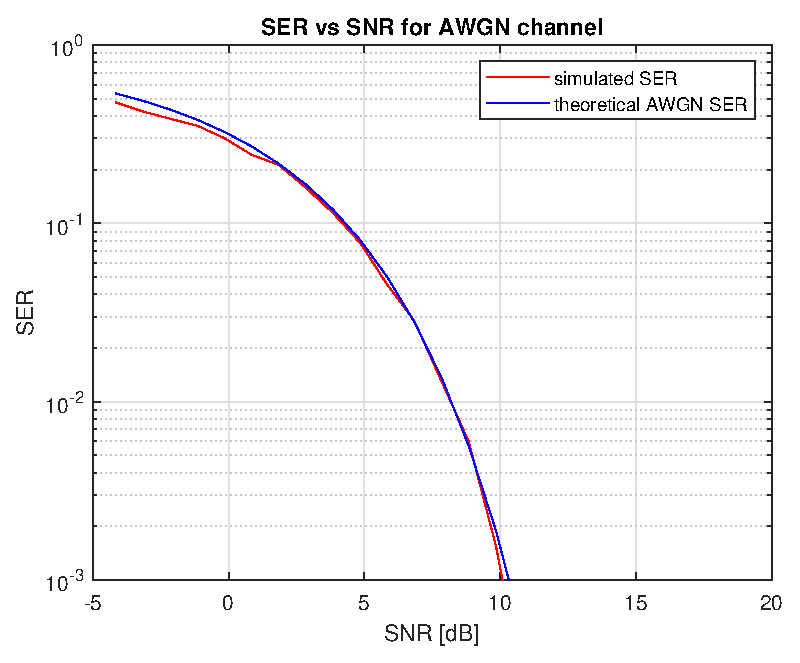
\includegraphics[width=\linewidth]{images/SERvsSNR_awgn.eps}
    \caption{Plot of simulated and theoretical SER vs SNR over the AWGN channel}
    \label{SERawgn}
\end{figure}

As can be seen in figures \ref{SERfading} and \ref{SERawgn} the worst value of the SER is about 0,5, which corresponds to the same probability that a random guess would be for the QPSK. Something else that can be noticed in figure \ref{SERawgn} and \ref{SERfading} is that the transmission over the AWGN channel performs better than the Fading channel and for some reason even better than the theoretical one. This is expected since the theoretical values corresponds to an ideal case, and the AWGN channel is the same as the fading channel but without the effects of shadowing and multipath.


\subsection{Analysis of cyclic prefix}
The cyclic prefix is generated to prevent ISI and Inter Carrier Interference (ICI). At the same time, keep the orthogonality between sub-carriers. The length of cyclic prefix ($N_{cp}$) will effect the transmission rate and its performance. 

The effect of the cyclic prefix can be studied in Appendix \ref{SCA_cp} where a comparison between figure \ref{Ncp0}, that is a scatter plot when no cyclic prefix is used, compared to the figure \ref{Ncp5}, were the it is long enough. Then it can be observed that the cyclic prefix delivers a tighter grouping round the constellation point compared to figure \ref{Ncp0}.

In figure \ref{SERncp} the correlation between SER and $N_{cp}$ for a specific SNR is illustrated. Here it is even more clear that a to short prefix will in the end generate errors. 

A longer cyclic prefix will make the communication system more robust against larger delay spreads of the channel. However, the transmission rate will suffer for it, since the length of the OFDM symbol is fixed.

If the value of $N_{cp}$ is too small, the previous OFDM symbol could leak into the current OFDM symbol which means that it does not eliminate interference anymore. This in turn is only waste of space, since it does not improve the transmission and still takes place from the actual information that is transmitted.  

\begin{figure}[H]
    \centering
    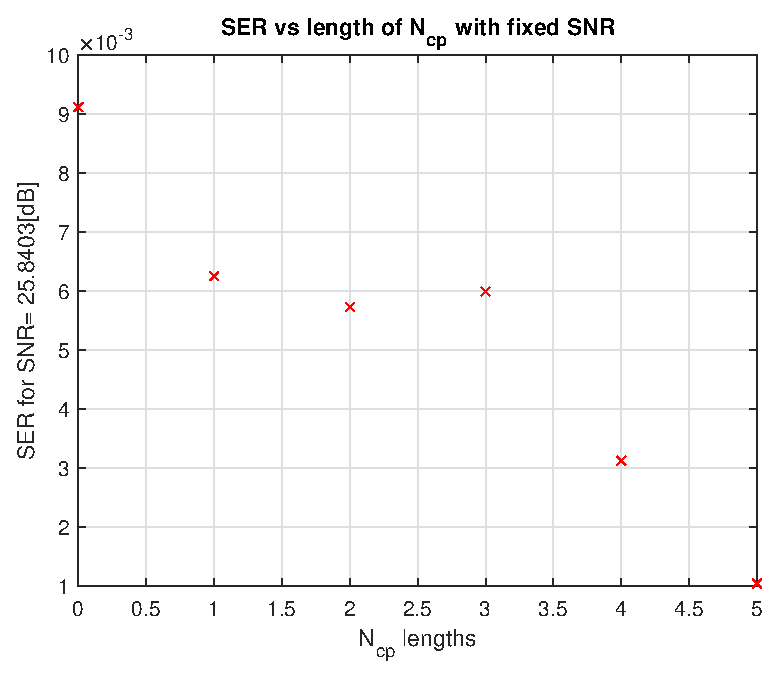
\includegraphics[width=\linewidth]{images/SER_Ncp.eps}
    \caption{SER with different value of $N_{cp}$}
    \label{SERncp}
\end{figure}


% add scatter plot and SER plot to do further explanation
%If the length of cyclic prefix is chosen as 2 rather than 5 as previous, there are more errors and the scatter plots look worse. Since $N_{cp}$ is too short to avoid interference between symbols and carriers. The scatter plots are shown in Appendix.
\section{Members contribution}
The way this part of the project was done was once again have all members try to figure out on their own how the MATLAB simulation part is to be implemented and then together discuss the solutions. In the end, the MATLAB code was mainly done by Oskar and Yuling. The text were mainly written by Erik, Yuling and Haitham. Oskar fixed most of the languages and all figures and some erroneous texts. 

 \clearpage
\begin{appendices}
\section{}
Here are the scatter plots of received symbols over AWGN channel with specific subcarriers. They are plotted with fixed length of cyclic prefix $N_{cp} = 5$ and a fixed $SNR = 25.84$ dB.
\label{SCA_AWGN}
\begin{figure}[H]
    \centering
    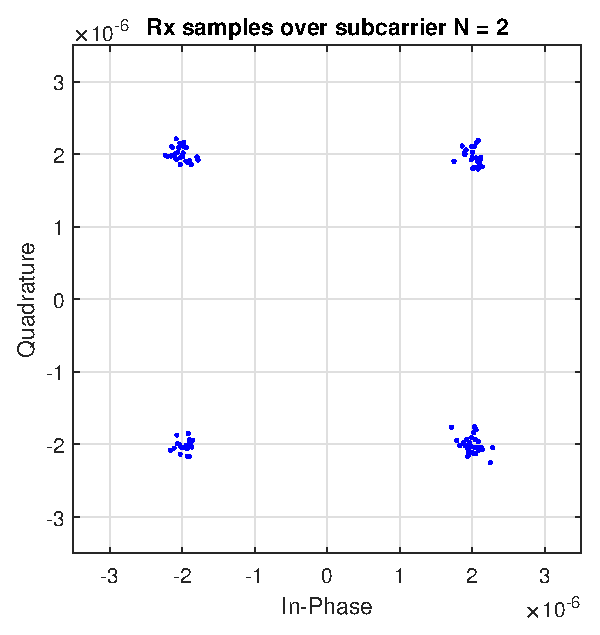
\includegraphics[width=\linewidth]{images/AWGNN2.eps}
    \caption{Scatterplot of samples transmitted over subcarrier \#2}
    \label{AWGN2}
\end{figure}

\begin{figure}[H]
    \centering
    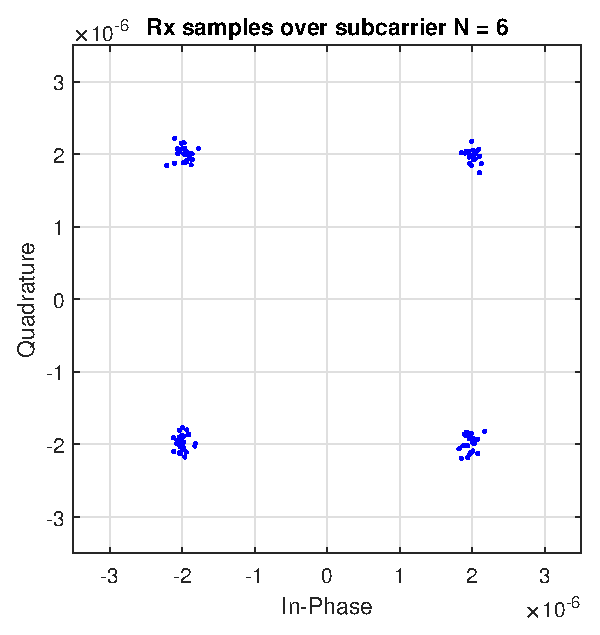
\includegraphics[width=\linewidth]{images/AWGNN6.eps}
    \caption{Scatterplot of samples transmitted over subcarrier \#6}
    \label{AWGN6}
\end{figure}

\begin{figure}[H]
    \centering
    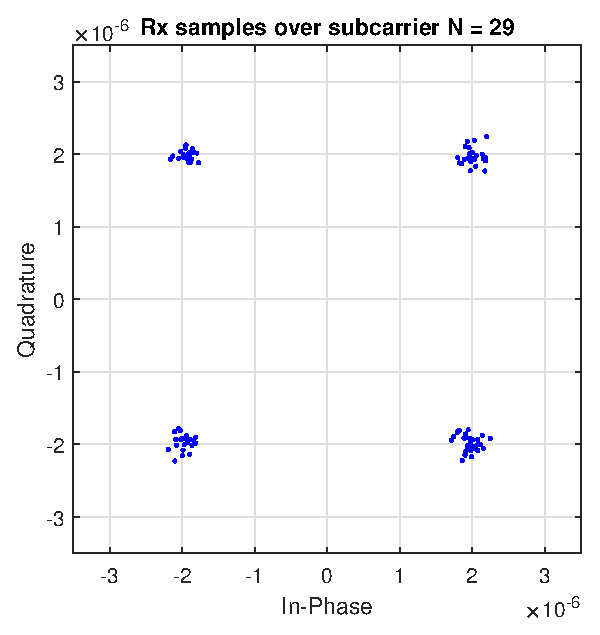
\includegraphics[width=\linewidth]{images/AWGNN29.eps}
    \caption{Scatterplot of samples transmitted over subcarrier \#29}
    \label{AWGN29}
\end{figure}

\begin{figure}[H]
    \centering
    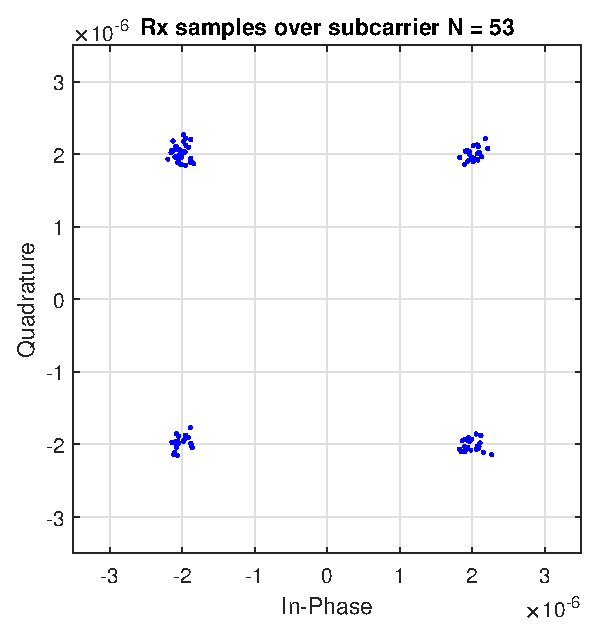
\includegraphics[width=\linewidth]{images/AWGNN53.eps}
    \caption{Scatterplot of samples transmitted over subcarrier \#53}
    \label{AWGN53}
\end{figure}

\begin{figure}[H]
    \centering
    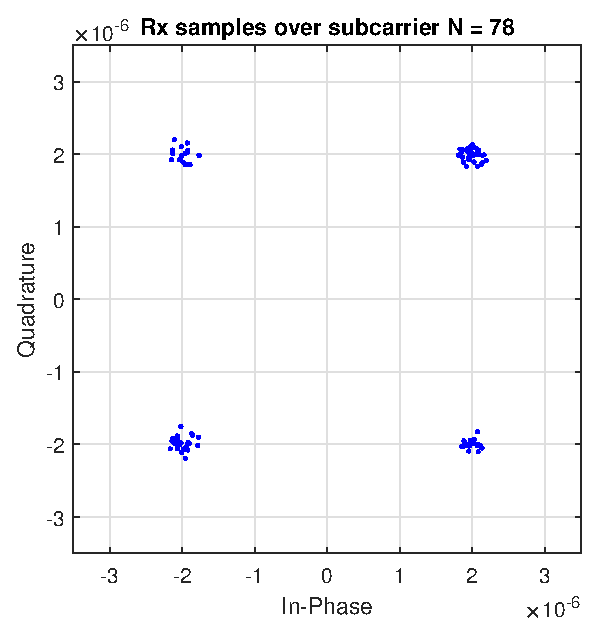
\includegraphics[width=\linewidth]{images/AWGNN78.eps}
    \caption{Scatterplot of samples transmitted over subcarrier \#78}
    \label{AWGN78}
\end{figure}

\section{}
\label{SCA_fading}
These scatter plots shows received QPSK symbols over fading channel with specific subcarriers. They are plotted with $N_{cp} = 5$ and a fixed $SNR = 25.84$ dB.

\begin{figure}[H]
    \centering
    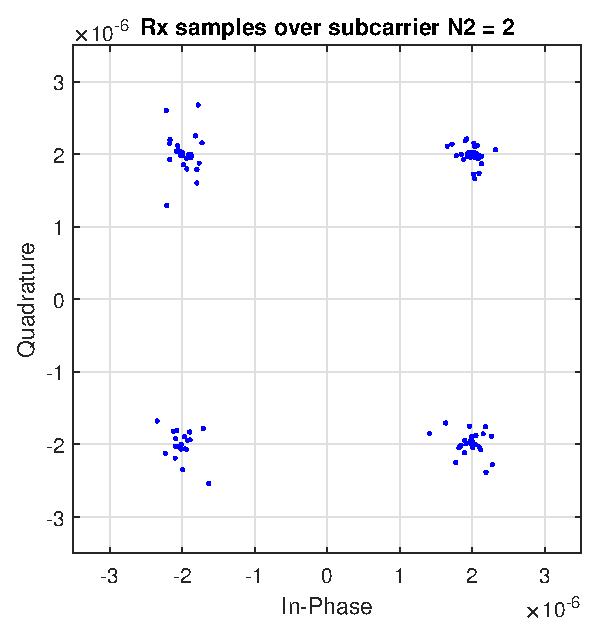
\includegraphics[width=\linewidth]{images/ScatterN2.eps}
    \caption{Scatterplot of samples transmitted over subcarrier \#2}
    \label{N2}
\end{figure}

\begin{figure}[H]
    \centering
    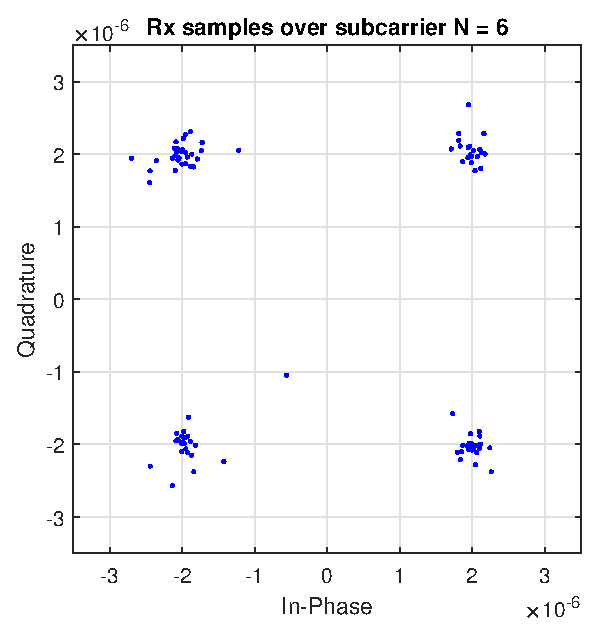
\includegraphics[width=\linewidth]{images/ScatterN6.eps}
    \caption{Scatterplot of samples transmitted over subcarrier \#6}
    \label{N6}
\end{figure}

\begin{figure}[H]
    \centering
    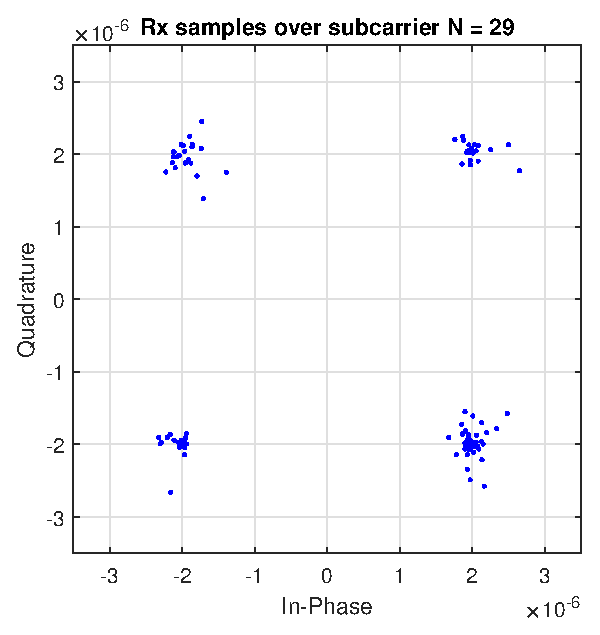
\includegraphics[width=\linewidth]{images/ScatterN29.eps}
    \caption{Scatterplot of samples transmitted over subcarrier \#29}
    \label{N29}
\end{figure}

\begin{figure}[H]
    \centering
    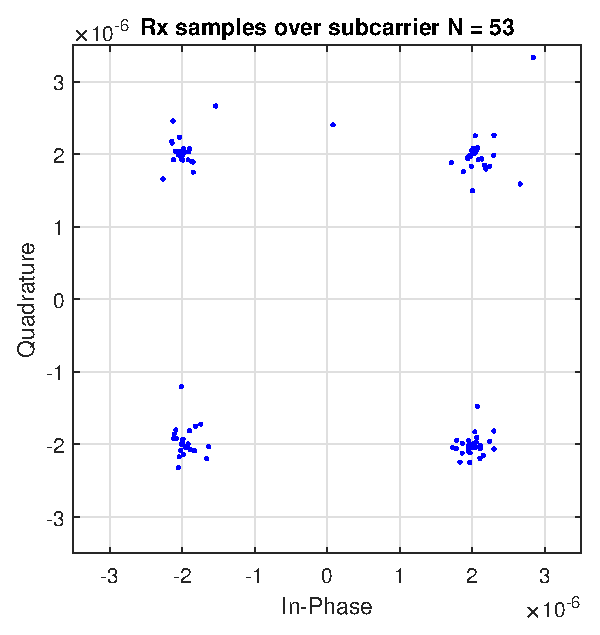
\includegraphics[width=\linewidth]{images/ScatterN53.eps}
    \caption{Scatterplot of samples transmitted over subcarrier \#53}
    \label{N53}
\end{figure}

\begin{figure}[H]
    \centering
    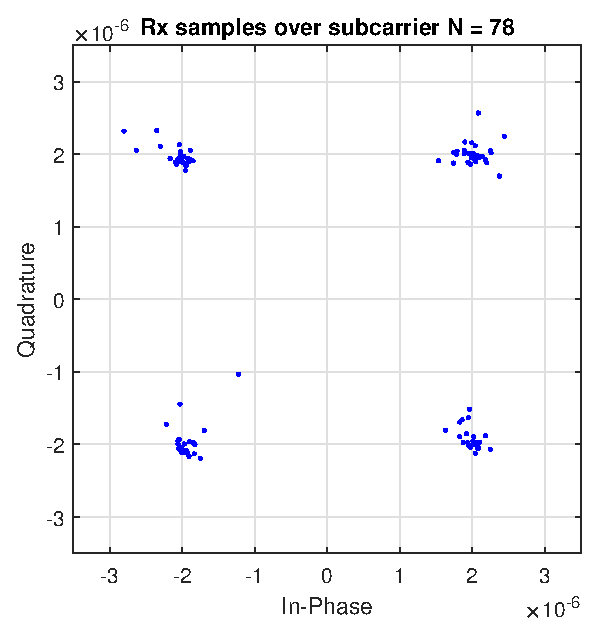
\includegraphics[width=\linewidth]{images/ScatterN78.eps}
    \caption{Scatterplot of samples transmitted over subcarrier \#78}
    \label{N78}
\end{figure}

\section{}
\label{SCA_cp}
Here are scatter plots with varying length of cyclic prefix.
\begin{figure}[H]
    \centering
    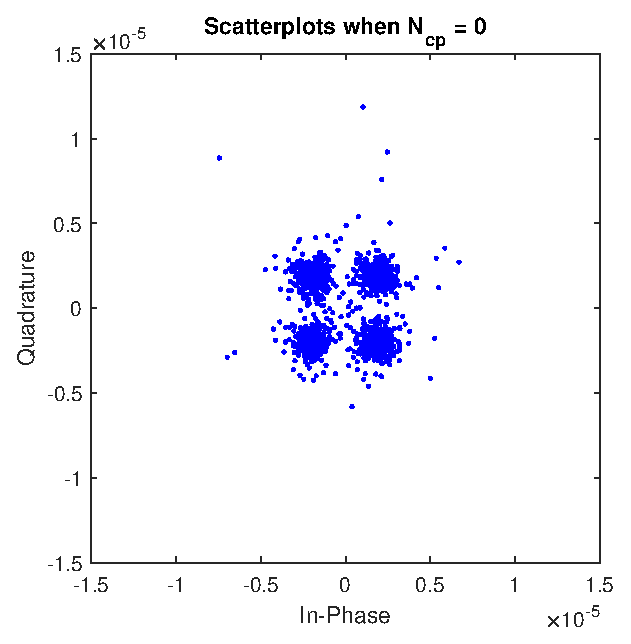
\includegraphics[width=\linewidth]{images/scatter_Ncp0.eps}
    \caption{Scatter plot with $N_{cp} = 0$}
    \label{Ncp0}
\end{figure}

\begin{figure}[H]
    \centering
    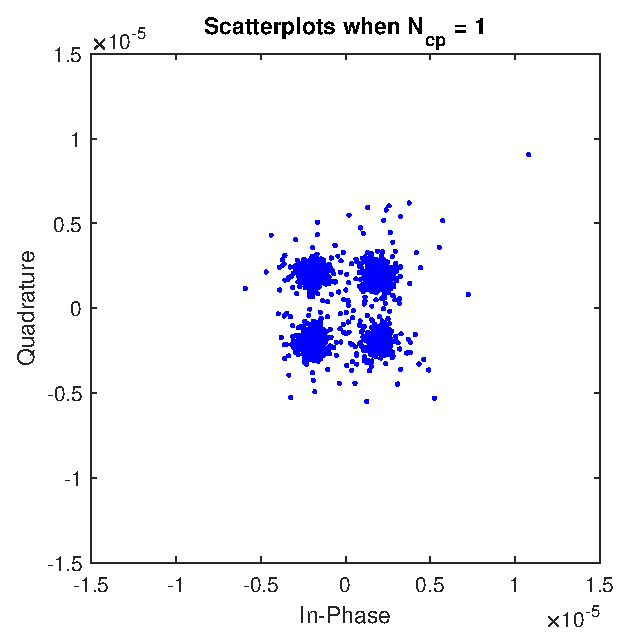
\includegraphics[width=\linewidth]{images/scatter_Ncp1.eps}
    \caption{Scatter plot with $N_{cp} = 1$}
    \label{Ncp1}
\end{figure}

\begin{figure}[H]
    \centering
    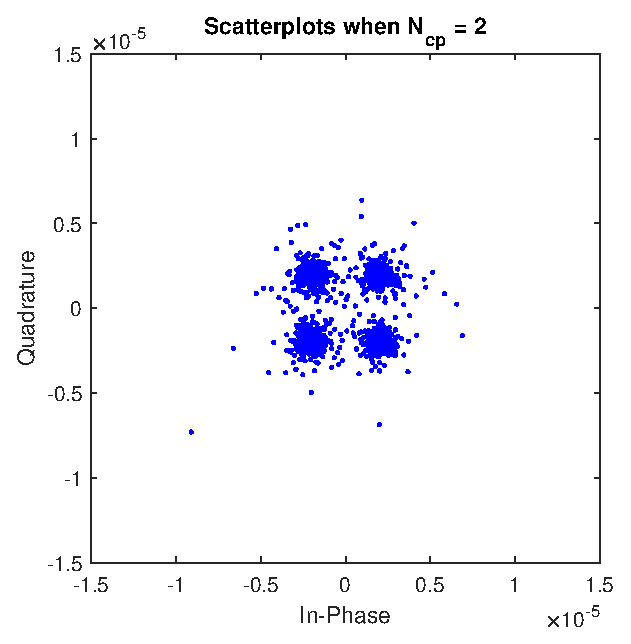
\includegraphics[width=\linewidth]{images/scatter_Ncp2.eps}
    \caption{Scatter plot with $N_{cp} = 2$}
    \label{Ncp2}
\end{figure}

\begin{figure}[H]
    \centering
    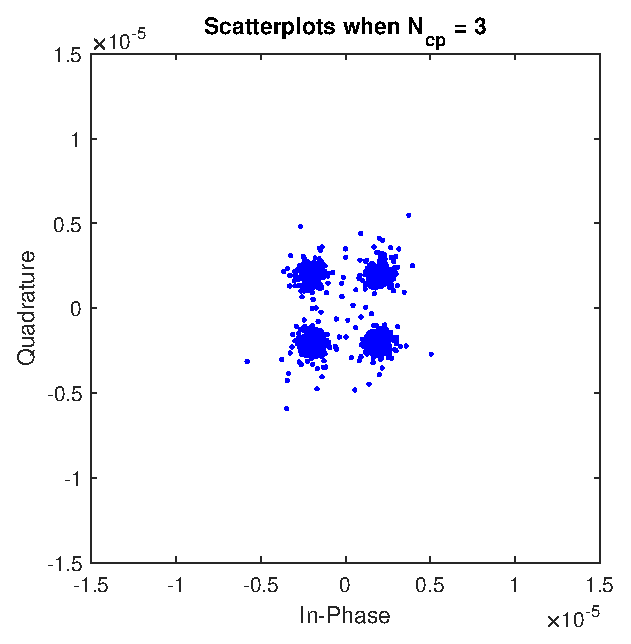
\includegraphics[width=\linewidth]{images/scatter_Ncp3.eps}
    \caption{Scatter plot with $N_{cp} = 3$}
    \label{Ncp3}
\end{figure}

\begin{figure}[H]
    \centering
    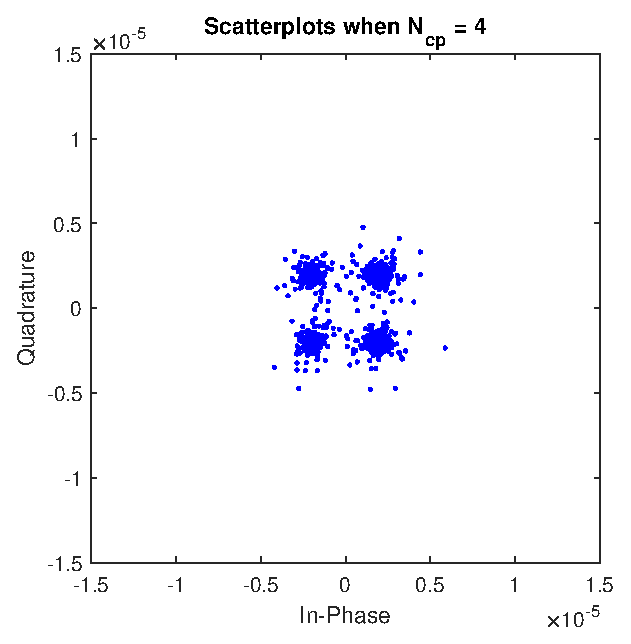
\includegraphics[width=\linewidth]{images/scatter_Ncp4.eps}
    \caption{Scatter plot with $N_{cp} = 4$}
    \label{Ncp4}
\end{figure}

\begin{figure}[H]
    \centering
    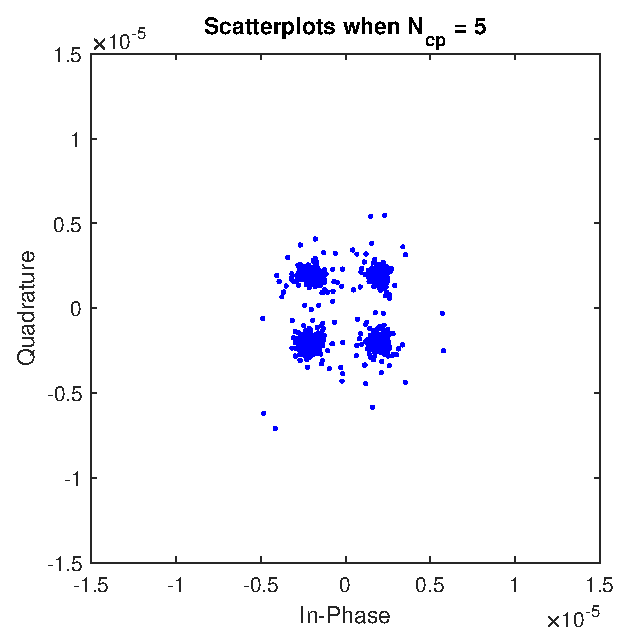
\includegraphics[width=\linewidth]{images/scatter_Ncp5.eps}
    \caption{Scatter plot with $N_{cp} = 5$}
    \label{Ncp5}
\end{figure}


\newpage
\section{}
    Here the MATLAB code written by the authors are given.
    

\lstset{language=Matlab,%
    %basicstyle=\color{red},
    breaklines=true,%
    morekeywords={matlab2tikz},
    keywordstyle=\color{blue},%
    morekeywords=[2]{1}, keywordstyle=[2]{\color{black}},
    identifierstyle=\color{black},%
    stringstyle=\color{mylilas},
    commentstyle=\color{mygreen},%
    showstringspaces=false,%without this there will be a symbol in the places where there is a space
    numbers=left,%
    numberstyle={\tiny \color{black}},% size of the numbers
    numbersep=9pt, % this defines how far the numbers are from the text
    emph=[1]{for,end,break},emphstyle=[1]\color{red}, %some words to emphasise
    %emph=[2]{word1,word2}, emphstyle=[2]{style},    
}


\lstinputlisting{MATLAB/projPart2.m}


\end{appendices}


\end{document}
